\documentclass[10pt,twocolumn]{article}

% use the oxycomps style file
\usepackage{oxycomps}

% usage: \fixme[comments describing issue]{text to be fixed}
% define \fixme as not doing anything special
\newcommand{\fixme}[2][]{#2}
% overwrite it so it shows up as red
\renewcommand{\fixme}[2][]{\textcolor{red}{#2}}
% overwrite it again so related text shows as footnotes
%\renewcommand{\fixme}[2][]{\textcolor{red}{#2\footnote{#1}}}

% read references.bib for the bibtex data
\bibliography{references}

% include metadata in the generated pdf file
\pdfinfo{
    /Title (Using Robotics To Make Blinds Smarter)
    /Author (Maryo Botros)
}

% set the title and author information
\title{Using Robotics To Make Blinds Smarter}
\author{Maryo Botros}
\affiliation{Occidental College}
\email{mbotros@oxy.edu}

\begin{document}

\maketitle

\section{Introduction and Problem Context}

Smart home technology has been developing rapidly, and many consumers have felt compelled to adopt this technology into their homes to help improve their way of living. This has especially been the case since the onset of the Covid-19 pandemic, when people have started to spend more time at home \cite{Ghosh2021SmartHomeDevice}. Examples of these tools include smart locks that can lock and unlock based on the user's location and smart lights that can turn on and off depending on whether or not a person is detected in a room. These devices often use automation in some capacity, to perform the tasks that humans normally would and are meant to enhance a user’s experience, while still fundamentally functioning in a familiar way.

Although this technology has gained more widespread adoption, there are still some areas of smart home technology that have yet to see development, namely, window blinds There are currently no mainstream smart home technology manufacturers that produce automated window blinds and yet blinds have great potential for improvement with automation. Blinds may seem simple because they are either opened or closed, but the ways people interact with them can be quite nuanced and reveal that automating blinds can bring significant improvements. Firstly, blinds can be automated to function as natural alarm clocks, automatically opening when the sun comes up. They can also be automated to automatically close when the sun sets, functioning as a privacy tool, as this is a time when people outside can see through a window. They can be automated to close at high temperatures to keep indoor temperatures cooler, which can save energy. Automated blinds can also allow a user to monitor their blinds remotely from an app, offering peace of mind. Additionally, automated blinds can be beneficial as an accessibility tool for users, especially those with disabilities who may have difficulties adjusting blinds according to their needs. Based on all of these use cases, there can be a great benefit to automating blinds.

The goal of this project is to automate blinds, using robotics. In order to do this, a robot that uses sensors and a motor will be needed to get readings on stimuli in the environment such as light and temperature, and then affect the blinds in response. A website will also be needed to allow the user to view the status of the blinds remotely and give the user the option for setting different modes and settings for the robot. This paper discusses the process for creating a robot that automates blinds along with the website that will pair with it. This process involves developing the robot and website and conducting two rounds of user testing to improve it. In the end, an evaluation is conducted to assess the success of the project, by testing the functions of the robot and gauging users’ experience testing it out.


\section{Technical Background}
\subsection{Smart Home Technology and Blinds}
Smart Home is the integration of technology and services through home networking for a better quality of living \cite{Hayes2022SmartHome}. These are devices that can cover many aspects of a home such as lighting, security, and heating, to name a few. Some smart locks, for example, are able to lock and unlock as a user walks up to a door. Often these smart home devices have some sort of app that allows a user to adjust settings or remotely interact with the smart home device in some way over an internet connection. Smart locks for example allow the user to lock and unlock a door remotely. These devices are meant to make the lives of a user better rather than more complicated. They should enhance a user’s life by making tasks more efficient or increasing accessibility without fundamentally changing the way they interact with a device or appliance \cite{Tamayo2022SmartHome}. They do not necessarily need to solve a problem but rather decrease the friction experience when doing everyday mundane tasks \cite{Tamayo2022SmartHome}.

There are many popular smart home devices such as security cameras, locks, and thermostats, however, one area of a smart home that currently lacks development is window blinds. In the year 2021, smart blinds did not appear on any list of the most popular smart home devices \cite{Woodall2021Popular}. Consumers are clearly interested in automating the tools and appliances they use at home and the lack of development with automated blinds, therefore, suggests that there have not been any compelling options offered yet.

Automated blinds currently have a lot of potential and many possible use cases. Automated blinds can serve as natural alarm clocks, automatically letting sunlight in a room as soon as the sun rises. They can be used as privacy devices, automatically closing when the sun goes down, which is the time when people usually turn lights on in the home and this would therefore compromise privacy as the indoors could be seen from the outside. Because of these two use cases, one way the blinds could be automated is by sensing light, opening when sunlight is detected, and shutting when it is not. Additionally, automated blinds can be closed when temperatures outside get too high, which would help keep indoor temperatures lower. This could also help reduce the amount of energy used for cooling down a room. Keeping a house cooler can significantly decrease the cost of energy and this could have even greater implications for commercial buildings that have dozens or hundreds of windows. Automated blinds can also offer a user peace of mind as the user can view the status of the robot and see whether the blinds are open or closed, remotely from an app. A use case for this could be if a user is not at home and wants to see if they made sure to shut the blinds before they left home. Although having blinds opened when not at home may not pose as great of a problem as leaving a door unlocked, for instance, it can still potentially be a security or privacy issue. Finally, automated blinds could function as an accessibility tool, especially for people who may suffer from disabilities, as they make it less necessary for a user to open and close the blinds manually, on their own.

In order to serve all of these use cases, a robot as well as an accompanying web application will be necessary. The web application will be needed to allow the user to see the status of the blinds as well as select between varying modes that use either light or temperature to automate the blinds. The robot, which will be referred to as the "blinds robot" for the purpose of this paper, will be a device that can be retrofitted on a set of blinds. This robot will be able to sense light and temperature levels and use a motor to move the blinds. For the purpose of this project, no mechanical parts will be developed to physically attach the motor to the blinds as that is beyond the scope of this project.

\subsection{Project Architecture}
The robot for this project will be developed using an Arduino microcontroller. Arduino is an open-source hardware and software company and they manufacture the controller for the robot, which is like the brain of the robot and will be discussed later in this section. The robot will need to be able to communicate with the web application and there is no way to directly communicate between an Arduino and a web page interface, but it is possible to facilitate a connection between them using a Node.js server that will pass messages back and forth \cite{Thomas2020Communicating}. In order to display the status of the robot, there needs to be a way to pass information from the Arduino to the webpage. Additionally, in order to select different modes so that the user can choose between what sensors they want to use on the Arduino, from the webpage, there needs to be a way to pass information from the webpage to the Arduino. The way these two processes will work is shown in Figure 1. The webpage will send information  back and forth with Node.js using socket.io and the Arduino will send information back and forth with Node.js using serialport. Socket.io is a library that enables real-time, bi-directional communication between clients and servers and serialport is a serial communication interface used in Arduino \cite{Fitzgerald2015Arduino}.

\begin{figure}
    \centering
    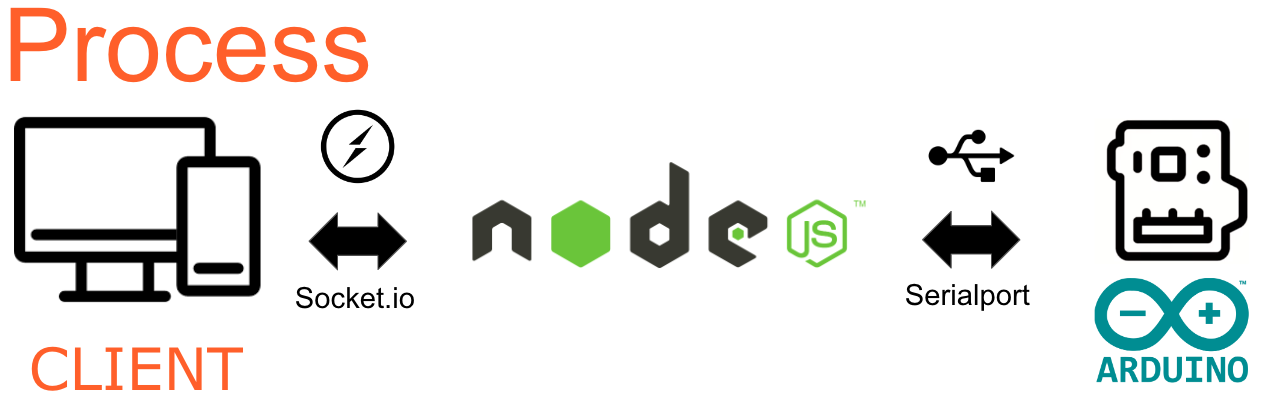
\includegraphics[width=.95\linewidth]{Figure 1.png}
    \caption{
        Architecture overview for the project.
    }
    \label{fig:fig1}
\end{figure}

\subsection{Robot}
The robot is a major component of this project, so it is important to discuss the requirements for a robot. Robotics is a quickly evolving field whose definition has been changing over time. A lot of the time, when people think of robots, they imagine metal, human-like machines trying to do human tasks. Although they don’t usually come in this form factor, oftentimes they are created to do menial tasks in the place of humans. Computer scientist and roboticist, Maja Mataric defines a robot as an autonomous system that exists in the physical world, can sense its environment, and can act on it to achieve some goals \cite{Mataric2007TheRoboticsPrimer}. Although Mataric’s definition is quite broad, it succinctly encompasses all of the important and necessary qualifications for what makes something a robot and it can be broken down into a few key requirements. 

\subsubsection{Physical}
The first requirement for a robot is that it must fundamentally exist in a physical world, meaning that it has to deal with the unbendable physical laws and challenges of the physical world. Having a physical body is known as embodiment \cite{Mataric2007TheRoboticsPrimer}. According to Mataric, this is what makes robots a real challenge. The blinds robot is a physical thing because it has a body that is composed of all the components and it has to physically affect the blinds.

\subsubsection{Actuators and Effectors}
The robot affects the physical world through the use of actuators and effectors. Mataric likens effectors to legs, flippers, wings, and various other body parts that allow animals to move \cite{Mataric2007TheRoboticsPrimer}. These effectors use underlying mechanisms such as muscles and motors. Effectors are the parts of the robot that physically interact with its environment and the actuators are the muscles that power those effectors to move. For the blinds robot, the effector is the part of the servo motor that is attached to the blinds. The actuator is the servo motor, which is a type of geared motor that can only rotate 180 degrees \cite{Fitzgerald2015Arduino}. It is controlled by sending electrical pulses from the Arduino which tell it what position to move to \cite{Fitzgerald2015Arduino}.

\subsubsection{Sensors}
In order to perform any actions in the physical world, robots need to have an understanding of that physical world so that they can perform the appropriate actions and this is what sensors are for. Robots use sensors to perceive their environment and get information and they can then process and perform actions on this information. Mataric defines sensors as devices that allow the robot to perceive its physical environment to get information about itself and its surroundings \cite{Mataric2007TheRoboticsPrimer}. The blinds robot will need to be able to sense temperature and light levels in order to affect the blinds. In order to sense temperature, a tmp36 sensor will be used and in order to sense light levels, a phototransistor will be used.

\subsubsection{Controller and Autonomy}
A robot can use its sensors to perceive the environment and it can then act on what it perceives using its actuators and effectors, but only if it has some way of processing the information that the sensors provide and only if it has a way of telling the actuators to affect the environment in a specific way. In order to accomplish this, the robot needs to have a controller. Controllers provide the hardware and/or software that makes the robot autonomous by using the sensor inputs to decide what actions to take and then to control the effectors to execute those actions \cite{Mataric2007TheRoboticsPrimer}. Controllers play the role of the brain in the entire operation and the controller for the blinds robot is an Arduino Uno microcontroller. This microcontroller is a simple computer and it is the part of the robot that is programmed. Mataric highlights that a robot is an autonomous system meaning that it acts on the basis of its own decisions, and is not controlled by a human \cite{Mataric2007TheRoboticsPrimer}. Although the blinds robot will need some user input from the webpage such as which mode it should use, it overall works autonomously, detecting sunlight and temperature levels, processing the information, and then taking appropriate actions, without any human intervention.

\subsubsection{Achieving Goals}
A true robot must act autonomously and exist physically to sense its environment, in order to accomplish goals. According to Mataric, we expect a true robot to have one or more goals and to act so as to achieve those goals \cite{Mataric2007TheRoboticsPrimer}. The goal of the blinds robot is to automate blinds according to the mode it is set in. For example, if it is in the temperature mode, its goal is to get temperature readings, and then if that temperature is above a certain threshold, the robot should close the blinds, otherwise, it should open them.


\section{Prior Work}
\subsection{Overview}
Although there are no mainstream smart home manufacturers offering blinds that are automated, there are still some projects that are similar to this one in some capacity. Three examples of prior work that will be discussed are motorized blinds, SwitchBot’s Blind Tilt, and an Arduino smart home light switch controller. 

\subsection{Motorized blinds}
The most popular products that share similarities with the blinds that were created for this project are motorized blinds. Several companies manufacture these blinds and often advertise them as “smart blinds.”Smart blinds are window coverings that can be opened or closed through an app or a voice commands on a smartphone. They come in various styles, such as accordion, slat, honeycomb, roller, and light filtering \cite{Alina20228BestSmartBlinds}. These blinds would not be considered robots because they do not use any sensors and so they are not automated in any way, which sets them apart from this project, as the focus of this project is controlling blinds autonomously. Additionally, these products are the complete blinds set, whereas this project focuses on a robot that can be attached to any existing set of blinds to retrofit them. Where motorized blinds share some similarities with this project is that they both have some sort of way to connect to the blinds over the internet. The motorized blinds can be set to open or close from an app on a smartphone and for this project, the blinds can also be set to open or close from the  web app.

\subsection{SwitchBot Blind Tilt}
The prior work that shares the most similarities to this project is a blind titling robot that is made by a company called SwitchBot. SwitchBot is a company that manufactures smart home technology at affordable prices, to make home appliances more interactive and fun \cite{SwitchBot2022}. The device is a robot that can be used to sense sunlight to open and close blinds and is attached to the wand of horizontal blinds \cite{WonderTechLab2022SwitchBot}. The device is powered using a solar panel and can be controlled to open and close from an app. A user can also use smart home assistants such as Amazon’s Alexa, Google Home, and Siri \cite{WonderTechLab2022SwitchBot}. There are a lot of similarities between this project and SwitchBot’s blind tilt. They are both robots that use sensors, specifically to measure sunlight to affect the blinds. They are also both built to be retrofitted on an existing set of blinds. Additionally, they both have some way of communicating with the robot over an internet connection. SwitchBot has an app that is associated with the device and for this project, there is a web app that connects with the robot. A difference between their two interfaces for interacting with their robots is that SwitchBot’s app allows the user to set schedules for opening and closing the blinds, while the website for this project does not incorporate any scheduling feature. Another difference between this project and SwitchBot’s Blind Tilt is that SwitchBot’s Blind Tilt only uses a sensor that detects light, meanwhile for this project, there are other sensors that are employed such as a temperature sensor and a potentiometer, which additionally allows the user to employ a combination of light and temperature sensors in automating the blinds from the web app, which Blind Tilt does not offer. 

\subsection{Arduino Remote Control Light Switch}
There are many similar smart home-related projects that others have made using Arduino, one of which is a remote-controlled light switch. The Remote Control Light Switch is a device that mounts over an existing light switch and uses a servo motor to turn the light switch on and off \cite{MerrittRemoteControlLightSwitch}. A pair of radio transceivers, one in the device itself and one in the remote allow the user to control the light remotely \cite{MerrittRemoteControlLightSwitch}. Like this project, the Arduino remote Control Light Switch is a device that is created using an Arduino microcontroller and it is created to retrofit an already existing appliance or tool; the remote control light switch is built to be placed on a light switch and the robot for this project is built to attach to the wand of a set of blinds. They both also give users the ability to remotely interact with the appliance, albeit in different fashions. The light switch can be remotely controlled using a button on another Arduino, meanwhile, the robot for this project can be remotely controlled from a web app. Another difference is that the remote control light switch is not a robot because it is not automated in any way.


\section{Methods}
\subsection{Using Light and Temperature to Affect Blinds}
\subsubsection{Sending Data from Arduino to Webpage}
For the process of putting together this project, I had to first find a way to pass information between an Arduino and a webpage. After researching this topic, I found that there was no way to directly communicate between an Arduino and a webpage, but it is possible to do it using a Node.js server to pass information between the two. According to creative technologist and developer, Indira Knight, Node.js works really well with Arduinos. Using the serial port you can use the server to pass data from an Arduino to a web page and pass data from the web to an Arduino \cite{Knight2018ConnectingArduino}. Node.js is a runtime environment for executing JavaScript server code and it makes it possible to create routes to web pages, connect to localhost, connect to a database, and send data to web pages with JavaScript \cite{Knight2018ConnectingArduino}. Figure 1 shows  the architecture for the process using Node.js.

Once I knew that it was possible to pass data back and forth between an Arduino and a webpage I wanted to make a robot that would automate blinds in response to light, so that the blinds could open in the morning when the sun came up, to function as a natural alarm clock, and close at night, to increase privacy. I also wanted the webpage to display the current angle of the servo motor. The SwitchBot blinds also incorporated a light sensor to automate the blinds to  open and close in the same way. In order to do this I would have to program the Arduino to move a servo motor based on light levels in a room and then send the status of the servo motor to be displayed on the webpage. My first step was to put together the circuit. The components that are required for the circuit are the Arduino Uno, a breadboard, a servo motor, a phototransistor, a 220-ohm resistor, and jumper cables. Figure 2 shows the circuit, with the phototransistor connected to analog port A1. The servo motor is connected to digital pin 9. These are the ports that allow the Arduino microcontroller to communicate with the phototransistor and servo motor. Energy moves from the power to ground on the breadboard and in the process, power is sent through to all the components on the breadboard. The breadboard is used in electronics for prototyping; it is a way to attach components to an Arduino without soldering \cite{Fitzgerald2015Arduino}. The phototransistor is the sensor that is used here to get data on light levels in a room. The servo motor only moves 180 degrees, where when the motor has turned the complete 180 degrees, this would move the blinds to a completely open position and when the servo is turned to 0 degrees, this would move the blinds to a completely closed position. 

\begin{figure}
    \centering
    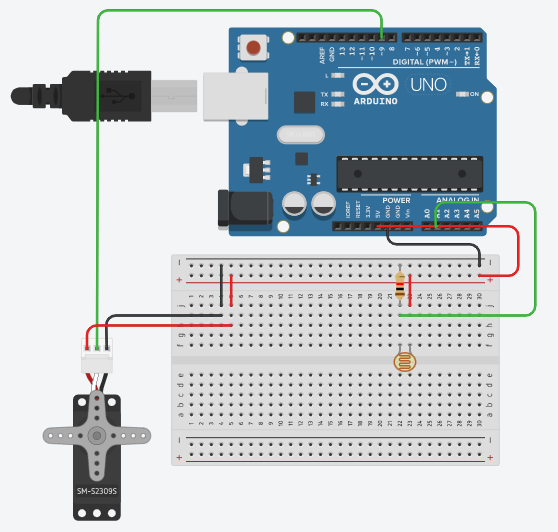
\includegraphics[width=.95\linewidth]{Figure 2.png}
    \caption{
        Arduino circuit with phototransistor and servo motor
    }
    \label{fig:fig2}
\end{figure}

After putting the circuit together, I wanted the blinds to open completely if light was sensed and close if there was no light. This would mean that if the phototransistor picked up light levels that were equal to or above a certain threshold, then the servo motor should move to 180 degrees and if it did not, then the servo should move to 0 degrees. After programming and then testing this out, I found out that it worked effectively. 

I next wanted to send the status of the servo motor to the webpage and display the angle there. As shown in Figure 1 the way that data is sent from the Arduino to the Node.js server is using the serial port. Data that is sent through the serial port can be seen in the serial monitor which enables me to report back results from the microcontroller like a console \cite{Fitzgerald2015Arduino}. The serial monitor is a great way to get information about the status of sensors and get an idea about what is happening on the circuit and the code as it runs \cite{Fitzgerald2015Arduino}. It is also how I can view what information is being passed from the Arduino to the webpage over the serial port. I added print statements to the serial monitor that indicated the angle of the servo. Figure 3 shows the serial monitor outputting the angle of the servo as it changes when light is shined on the robot and then when it is no longer shining on it. 

\begin{figure}
    \centering
    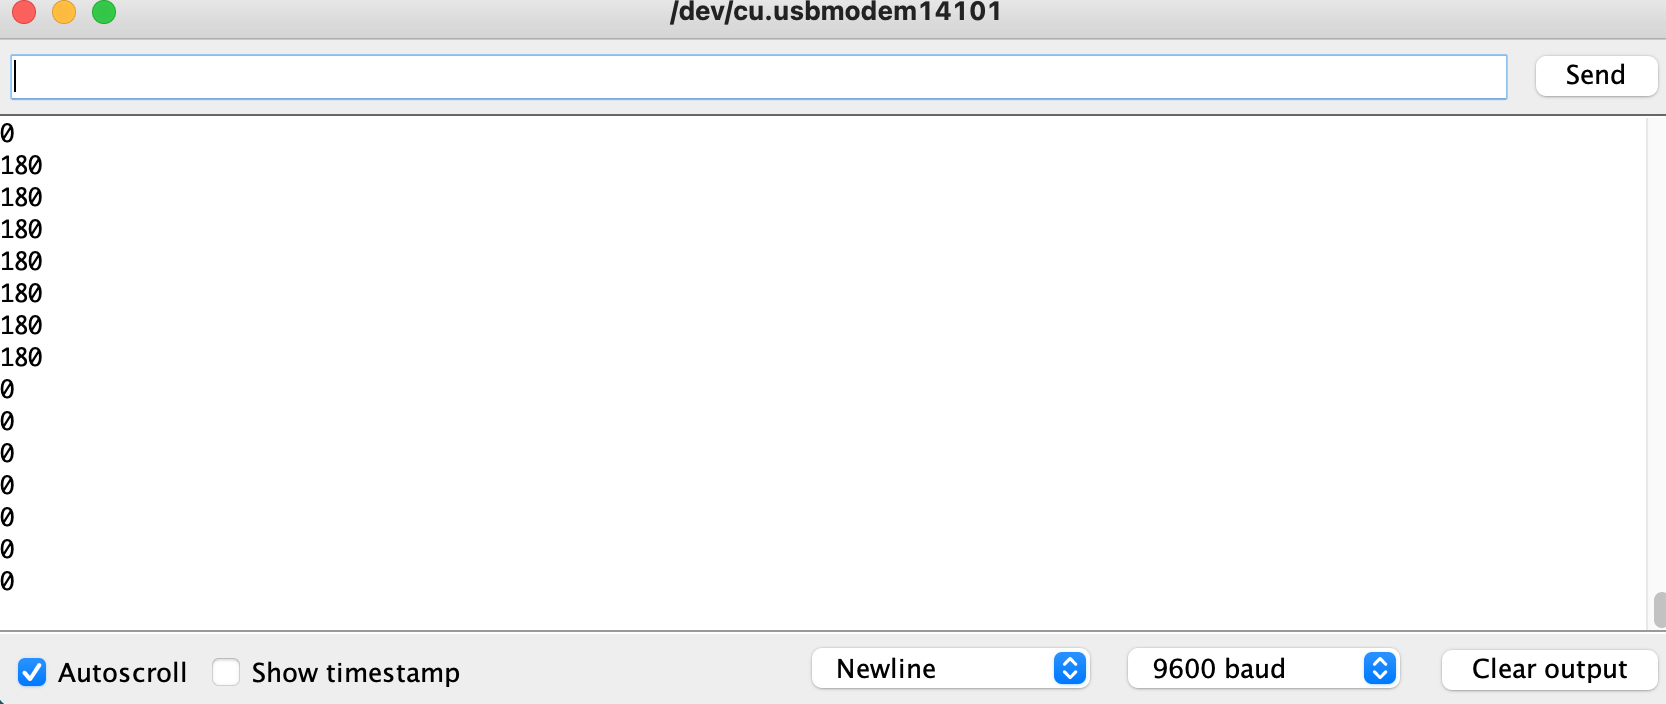
\includegraphics[width=.95\linewidth]{Figure 3.png}
    \caption{
        Serial monitor showing servo's angle changing from 0 to 180 and back to 0 again in reponse to changing light in the environment.
    }
    \label{fig:fig3}
\end{figure}

\subsubsection*{Sending Data From Webpage to Arduino}
I next wanted to test out sending data from the web page to the Arduino and in the process of doing this, I would also add a way to automate the blinds using temperature. I wanted to add two buttons to the webpage which would each select a mode. One mode would use the light sensor to automate the blinds based on light, and the other mode would automate the blinds based on temperature. Temperature is one of the methods I am using to automate the blinds because it can help keep a room cooler and save on energy costs when the blinds are closed at higher temperatures \cite{Jang2014ToStayCool}.

I began by adding a temperature sensor to the circuit. The specific sensor that was used is a tmp36 sensor, which has three prongs for a connection to power, ground, and the analog voltage, which is connected to analog pin A5, as can be seen in Figure 4. Once the circuit was put together, I next moved on to testing the sensor. The program written for testing the temperature sensor read the analog value of the temperature sensor and outputted it to the serial monitor. Testing the temperature sensor proved to be slightly more challenging than testing the phototransistor because it is harder to change the ambient temperature than it is to change ambient lightning. The way I was able to change ambient temperature was by directing a fan toward the sensor to make the temperature cooler and directing a heater toward it to make the temperature warmer. This method showed that the tmp36 sensor did pick up on the changes in temperature and Figure 5 shows the sensor’s readings on the serial monitor.

\begin{figure}
    \centering
    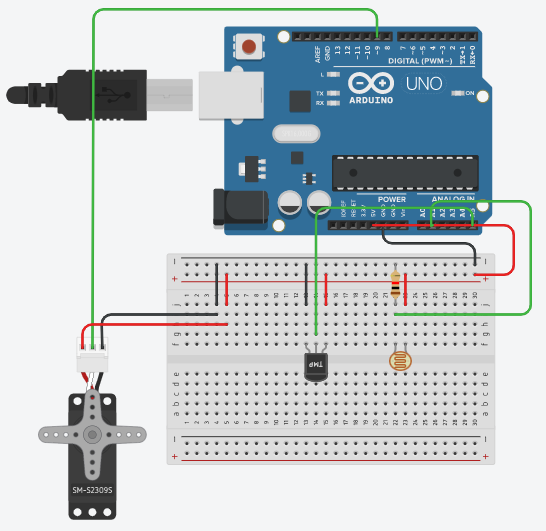
\includegraphics[width=.95\linewidth]{Figure 4.png}
    \caption{
        Arduino circuit with the addition of the tmp36 temperature sensor.
    }
    \label{fig:fig4}
\end{figure}

\begin{figure}
    \centering
    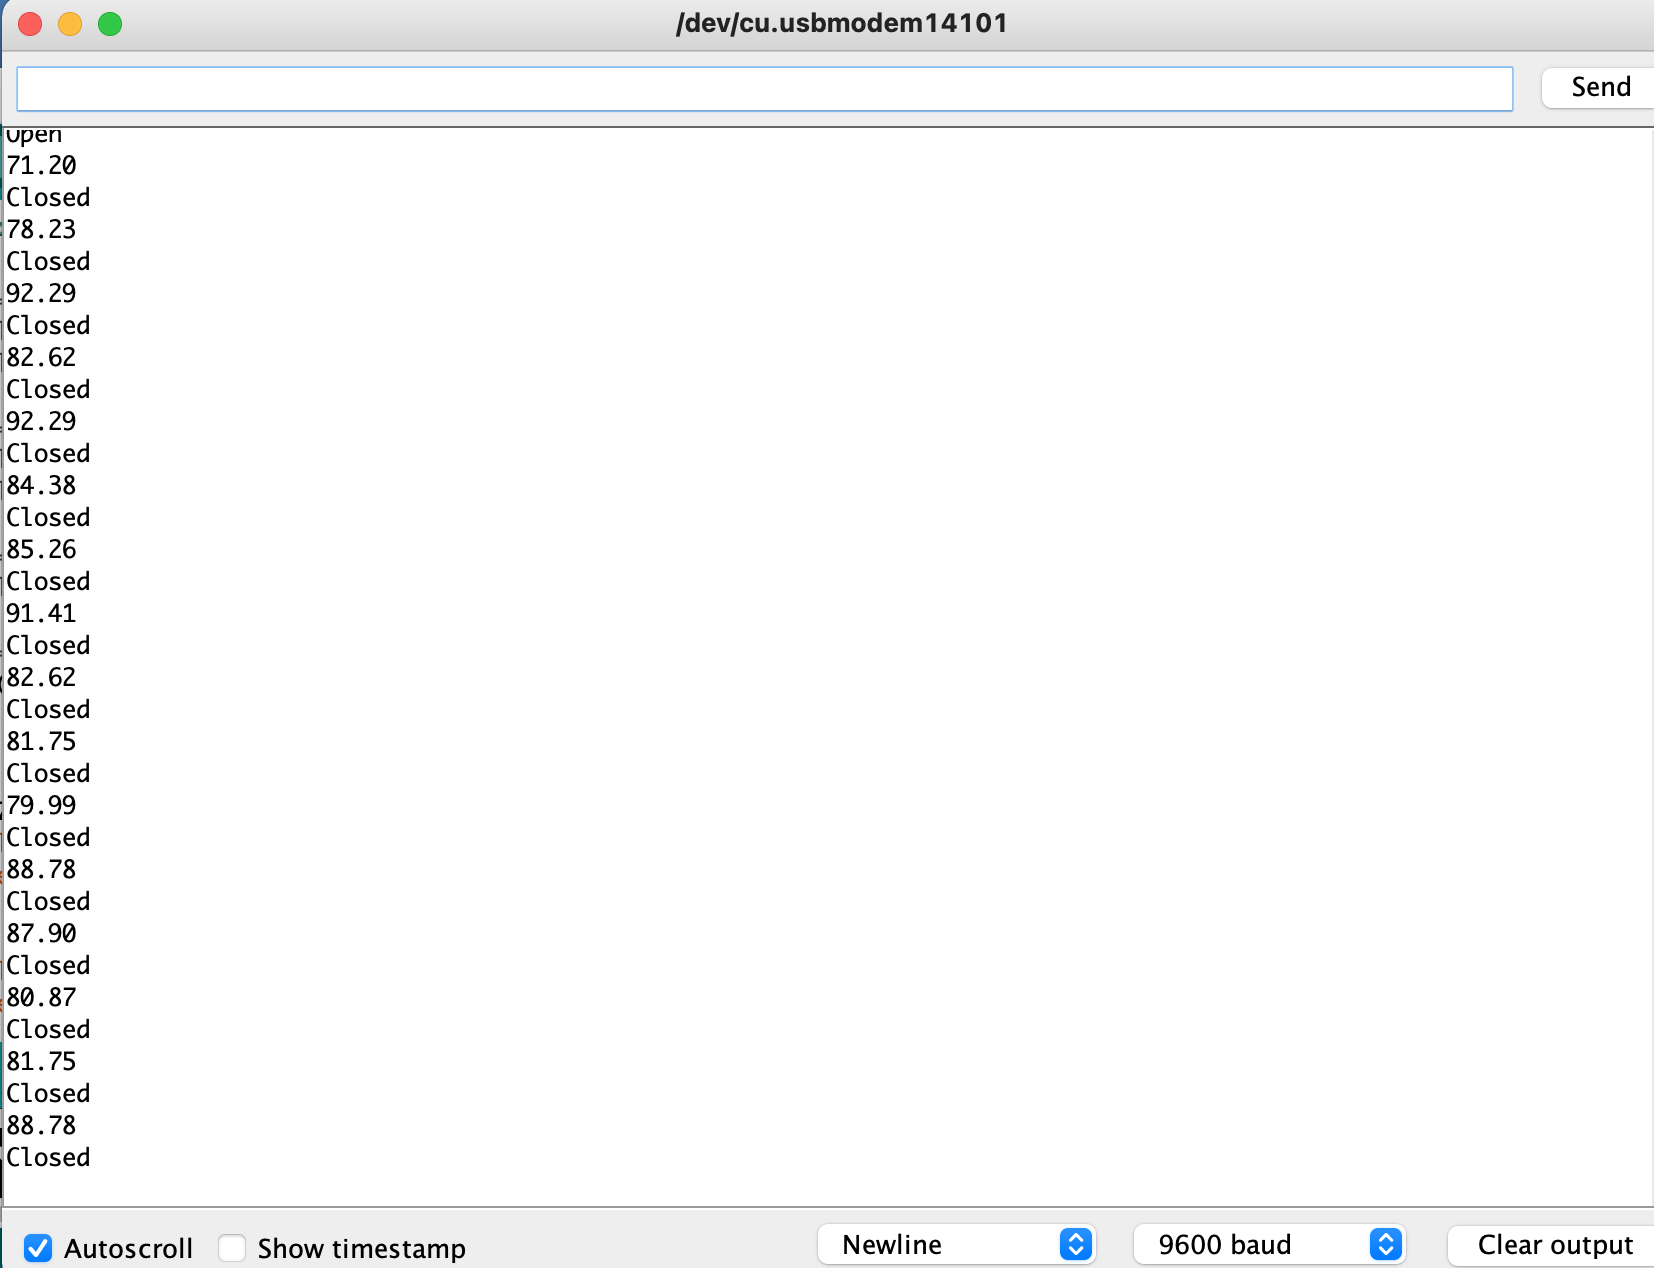
\includegraphics[width=.95\linewidth]{Figure 5.png}
    \caption{
        Serial monitor showing temperature changing as I briefly direct a heater at the sensor. 
    }
    \label{fig:fig5}
\end{figure}

For the second part of testing the temperature sensor, I wanted to use the temperature sensor in a similar way I used the phototransistor to affect the servo motor. I wrote the program so that the servo would move to 0 degrees if the temperature reached 90 degrees Fahrenheit or greater and would move to 180 degrees if the temperature was less than 90 degrees Fahrenheit. I used this threshold for testing purposes. This would mean that the blinds would be closed if the temperature reached 90 degrees or greater and would be closed otherwise.

At this stage, there were now two different ways of autonomously opening and closing the blinds: using temperature and light The next step is giving the user the ability to choose between these two methods of affecting the blinds through the webpage. On the webpage, I added the two buttons, labeled “Light Mode'' and “Temperature Mode.” When the user clicks one of these buttons, it sends a unique code to the Arduino using socket.io, indicating to it the appropriate function that should be executed: the function that uses the phototransistor to autonomously affect the servo or the function that uses the temperature sensor to autonomously affect the servo. 

\subsection{User Testing Round 1}
Once I got two modes working for the robot, light mode, and temperature mode, it was an appropriate time to conduct the first round of user testing to receive feedback. The way this was conducted was by taking a group of four individuals and explaining the goal of the project. Each user was then given 10 to 15 minutes to interact with the robot and website and then respond to a few open-ended questions as well as questions asking about potential desired features, that would gauge what worked and what didn’t work with the project so far, as well as what could be done moving forward. The organized responses to these questions can be found in UserTestingAndEvaluation.pdf. The questions are listed below:

\begin{itemize}
    \item \texttt What are some of the pain points of the project so far?
    \item \texttt What do you like about the project?
    \item \texttt Are you more likely to use a combination of light and temperature to automate blinds or would you just use one or the other?
    \item \texttt Is it important for you to see the status of the blinds?
\end{itemize}

\subsubsection{What users liked}
The results showed that all users were satisfied with the use of temperature and light to autonomously control the blinds. However, all users stated that they were more likely to combine temperature and light rather than exclusively use one or the other. This reveals that adding modes that possibly apply boolean logic to the temperature and light sensors will be a change that will have to be made.

\subsubsection{Need for status information on website}
All users pointed out that they wanted to have access to information about the status of the blinds, to see whether they were opened or closed. The only thing that was displayed at this stage was the angle of the servo, which was not very useful information for the user. Therefore, instead of sending 180 degrees or 0 degrees to be displayed on the website, I should be sending “open” or “closed.” The motorized blinds as well as the SwitchBot blinds that were mentioned in the prior work also displayed the status of the blinds on their apps and this was already a feature I planned on implementing. To take this further, another important piece of information that can be displayed on the webpage as well could be the mode that is currently being used.

\subsubsection{Pain Point: Lack of manual control}
Several users pointed out that having the robot attached to the blinds took away their ability to manually control the blinds themselves. Users wanted to have that ability to bring back the physical twisting of the wand. Using this feedback I knew I needed to add something that will give the user back the ability to manually control the blinds. The best smart home devices are the ones that enhance the user’s experience, without fundamentally altering the way they interact with the appliance or tool \cite{Tamayo2022SmartHome}. Although I had now enhanced the functionality of the blinds, making them operate autonomously based on light and temperature, I had removed the option to make manual adjustments. This is how users were accustomed to operating their blinds and therefore, this functionality needed to be brought back.

\subsection{Improvements After User Testing Round 1}
\subsubsection{4.3.1 Adding boolean logic modes}
Using what I had learned from the first round of user testing, I began by making the necessary improvements, starting with adding options for the user to apply boolean logic to customize the automation with the temperature and light sensor. To do this, I added two more buttons on the webpage for the two new modes. One of the modes will be denoted as “Temperature or Phototransistor.” When this mode is used, the blinds will open if either the temperature is greater than 90 degrees Fahrenheit or the phototransistor senses light. The second mode will be denoted as “Temperature and Phototransistor.” When this mode is used, the blinds will only close if both the temperature is greater than or equal to 90 degrees Fahrenheit and the phototransistor does not sense light. At this stage, there are now four modes: Temperature, Light, Temperature or Light, and Temperature and Light.

\subsubsection{Adding status indicators}
The next improvement after the first round of user testing is adding a status indicator on the webpage. This status indicator would be an area on the webpage that would let the user know which mode the robot is currently in. Additionally, instead of having the webpage display the angle of the servo motor, it would instead indicate “Status: Open” or “Status: Closed,” to let the user view the status of the blinds remotely. I added to this by also including the current mode that was selected by the user. With these additions, the webpage now gives the user information on the mode of automation and the status of the blinds.

\subsubsection{Adding a potentiometer mode}
The final improvement that had to be made after the first round of user testing was giving the user the ability to manually control the blinds. Two options initially came to mind for doing this: making a slider on the webpage or using a potentiometer as a dial that a user would be able to twist. I decided to go with the latter option since users explicitly indicated that the physical twisting was no longer available compared to before the robot was connected to the blinds. Most regular blinds have a wand that twists in order to open or close them. In order to most closely match the way the user was familair with interacting with the blinds, I decided a dial that would twist in a similar way to how the wand would have to be twisted, would be the most suitable way for the user to interact with the blinds. A potentiometer is a type of voltage divider. As the user turns the knob, they change the ratio of the voltage between the middle pin and the power and this change is read in as an analog input \cite{Fitzgerald2015Arduino}. The potentiometer will allow the user to twist it to the left to close the blinds or twist it to the right to open the blinds and the user can also set the blinds anywhere between 0 and 180 degrees as well.

I first began by adding the potentiometer to the circuit. I added the potentiometer to the breadboard and attached its three prongs to power, ground, and analog port A0 as can be seen in Figure 6. After making this addition to the circuit, my next step was to program the Arduino to move the servo motor to 180 degrees when the potentiometer is twisted to the right and move the servo motor to 0 degrees when the potentiometer is twisted to the left. The servo moves from 0 to 180 degrees, but the potentiometer accepts analog values which are from 0 to 1023, so I scaled the numbers which allowed the potentiometer to successfully move the servo when it is twisted.

\begin{figure}
    \centering
    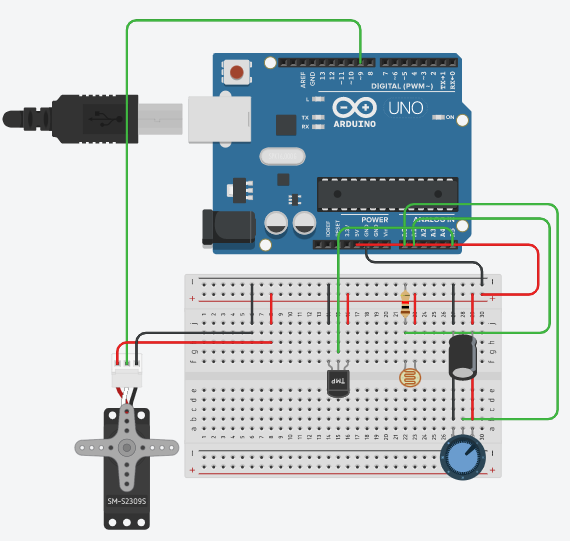
\includegraphics[width=.95\linewidth]{Figure 6.png}
    \caption{
        Arduino circuit with the addition of the potentiometer at the bottom right corner of the breadboard.
    }
    \label{fig:fig6}
\end{figure}

The final step was implementing this in the Arduino code for the project and adding a new mode for the user to select on the webpage. I added another button to the webpage, denoted as “Potentiometer Mode,” for the new mode. I implemented the potentiometer moving the servo into the Arduino code and for it to execute when the user selected the potentiometer mode. At this stage, there are now five modes in total with the addition of the potentiometer mode. Figure 7 shows the modes on the webpage by the end of this stage of the project.

\begin{figure}
    \centering
    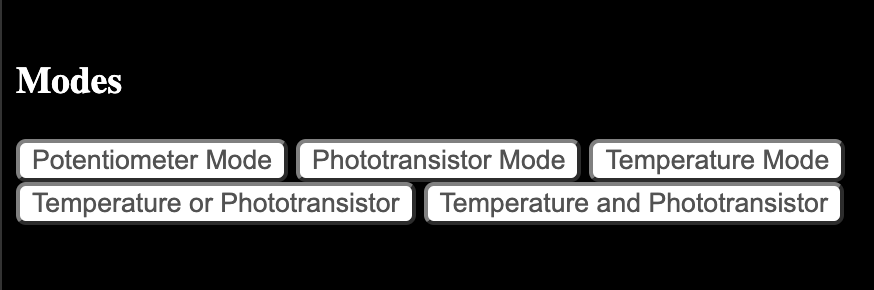
\includegraphics[width=.95\linewidth]{Figure 7.png}
    \caption{
        Modes section of webpage with buttons for all five modes. 
    }
    \label{fig:fig7}
\end{figure}

\subsection{User Testing Round 2}
After completing the improvements after the initial round of user testing, I conducted a second round to gauge whether or not I met the user’s needs and what other improvements could be made. The way this was conducted was similar to how the first round of user testing was conducted. I reiterated the goal of the project to the same group and each user was given 10 to 15 minutes to interact with the robot and website and then respond to a series of questions again. The organized responses to these questions can be found in UserTestingAndEvaluation.pdf. The questions are listed below:

\begin{itemize}
    \item \texttt What are some of the pain points of the project so far?
    \item \texttt What do you like about the project?
    \item \texttt Are the default thresholds for the sensors adequate or would it be better if the user could customize them?
\end{itemize}

\subsubsection{What users liked}
There were a few things users pointed out when it came to things they liked about the project. They liked the availability of different modes to choose from, for the customization of the automation. While most users agreed that the default threshold used for sensing sunlight worked properly all the time, most also agreed that they would like to set their own temperature threshold. So I knew now that I had to add some way for the user to enter their own custom temperature threshold as 90 degrees wouldn't suffice for all.

\subsubsection{Pain point: Blinds only completely open or completely close}
One of the pain points that users highlighted was that the blinds were restricted to opening completely or closing completely. This is because when the blinds are in an automated mode, the servo is only set to move to 0 degrees or 180 degrees, depending on what the sensors perceive in the environment. Users wanted to have the ability to customize the degree to which the blinds would close and open. This is a reasonable issue with the way the project is currently set up because not all users exclusively want to let as much light in as possible or let in the least amount of light possible. Users do often move their blinds to positions that are not necessarily completely open or completely closed.

Additionally, not all blinds are made the same and so 180 degrees on the servo can mean a completely different position for different blinds. This also brought to light that when the user is using the potentiometer mode, where they twist the dial to move the blinds, the status indicator on the webpage will indicate that the blinds are open if the servo angle is 90 degrees or greater and closed if it is less than 90 degrees, which may not be a suitable threshold for every set of blinds. Therefore, a threshold for the degree to which the dial has to be turned for when the blinds will be considered open or closed should also be something that the user should be able to customize as well. 

\subsubsection{Pain point: No way for user to open or close the blinds directly from the webpage}
One user pointed out that there should be an easy way to open or close the blinds directly from the webpage. In the first round of user testing, I identified that the user would want to regain manual control of the blinds so that they can open or close them at their will, but I opted for the option of putting a physical dial instead of a control on the webpage, in order to give the user a familiar way of interacting with the blinds. However, there are use cases where having the ability to also manually control the blinds from the web app may be useful. One example could be where the user may want to open or close the blinds remotely because the blinds are not within reach, or if the user is remotely monitoring the blinds and wants to also remotely open or close them.

\subsection{Improvements After User Testing Round 2}
\subsubsection{Adding temperature threshold customizability}
The first adjustment I made after the second round of user testing was to add a place where the user could enter a number they would like to set for the temperature threshold. I first started by adding an input box on the webpage and a button next to it, where the user could enter the temperature in degrees Fahrenheit and then click on the button to submit the change. This number is held in a variable and this variable  is used in the Arduino code for all of the modes that use temperature: Temperature mode, Temperature or Phototransstor mode, and Temperature and Phototransistor mode.

\subsubsection{Adding Settings for upper and lower limits and potentiometer threshold}
My next step was to allow the user to set the limits for the angle the servo should move to when the blinds should be considered closed or opened. I did this in a similar way to how I did the temperature threshold and potentiometer threshold inputs. I created input boxes on the web page with buttons that would allow the user to submit. At this point, there were a lot of input boxes for the user to make adjustments to thresholds and the limits for the servo. Because of this, I decided to consolidate them all into a “Settings” section on the webpage for a better user interface.

It is also important to point out that when a user enters a value in any of these input boxes, that value will be saved regardless of what mode they choose next. In other words, if a user enters 10 for the lower limit and they select the Temperature Mode and then switches to the Phototransistor Mode, this lower limit will remain the same and will not be reset just because the user selected a different mode.

\subsubsection{Adding buttons to open and close blinds}
The final adjustment I made after the second round of user testing was to add buttons on the webpage that would allow the user to directly open or close the blinds. This was a straightforward adjustment and I added two buttons, one for “Open” and the other for “Closed” and when each of these was clicked they would send a message to the Arduino to either set the servo to 180 degrees if “Open” was clicked or 0 degrees if “Closed” was clicked. Additionally, if the user set their own upper and lower limits in the Settings section, the servo would use these parameters for the angle to open or close to. Figure 8 shows the webpage after these changes.

\begin{figure}
    \centering
    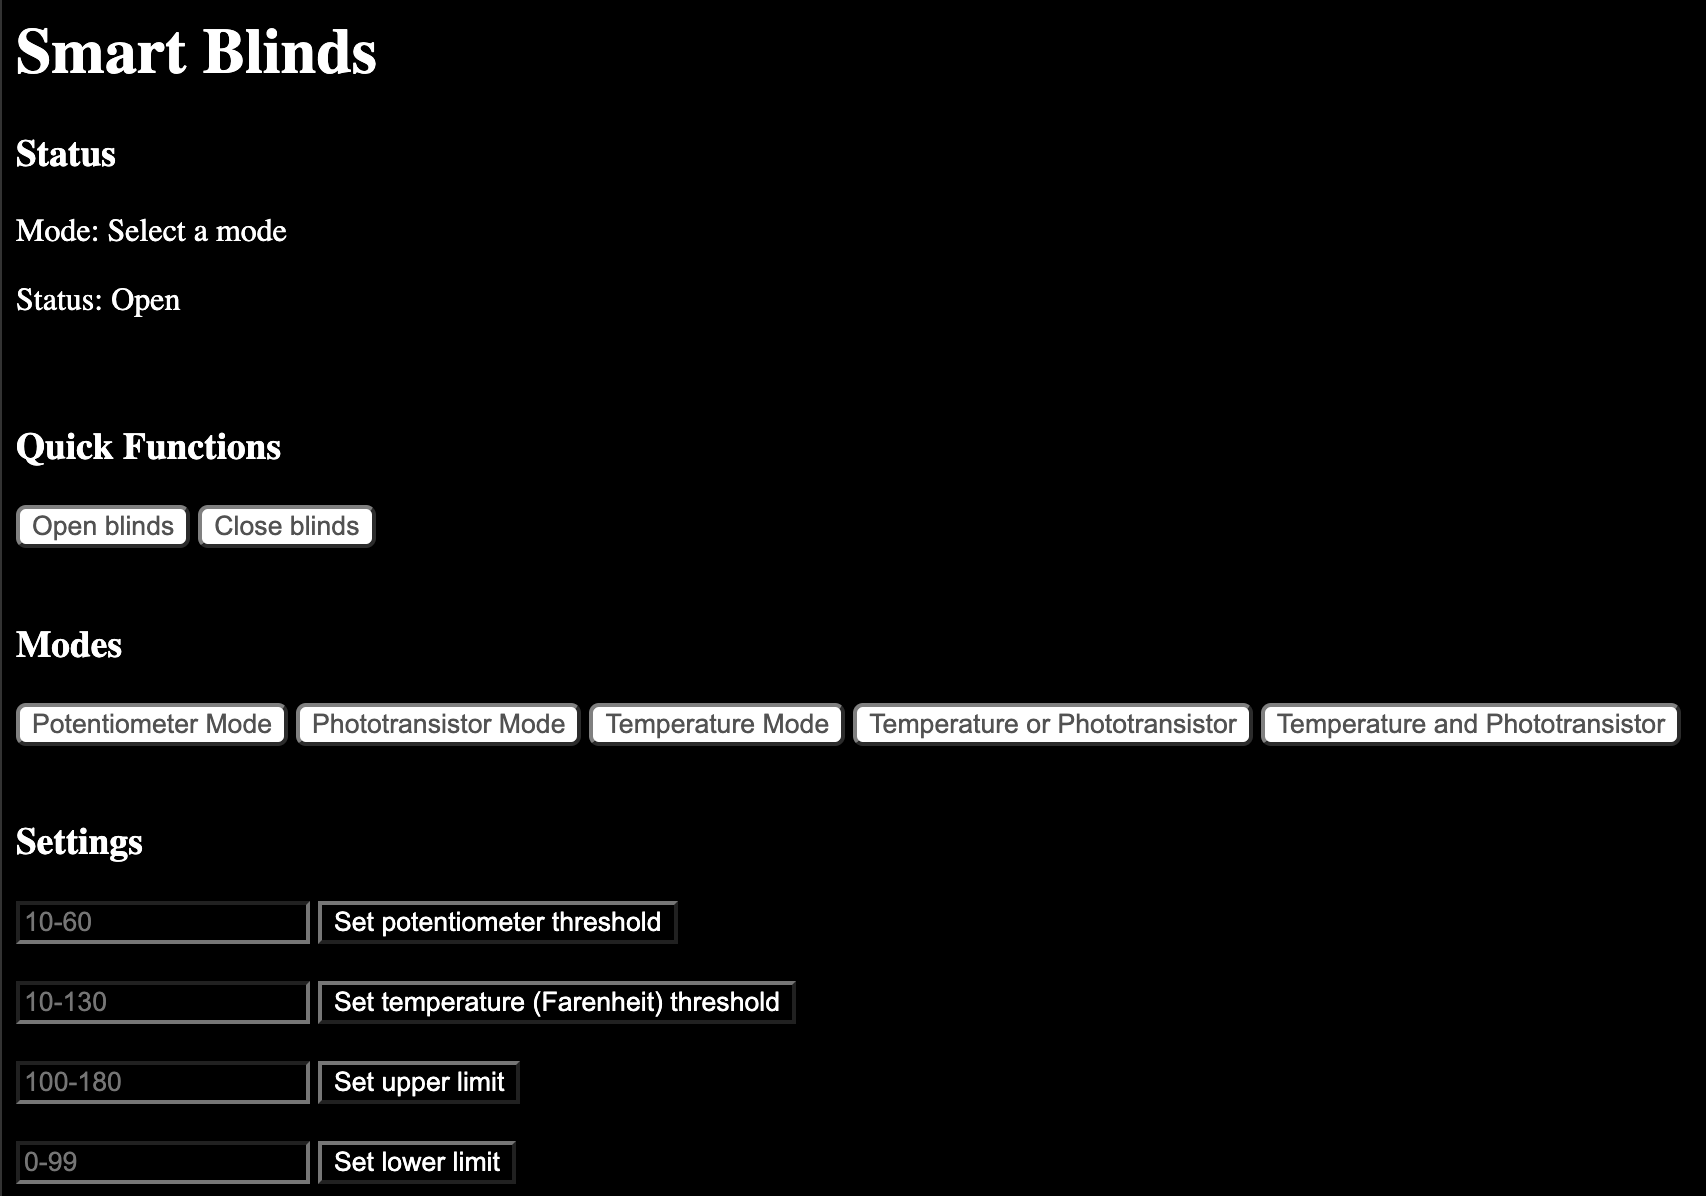
\includegraphics[width=.95\linewidth]{Figure 8.png}
    \caption{
        Final webpage UI with status section, quick functions section, modes section, and settings section.
    }
    \label{fig:fig8}
\end{figure}

\section{Evaluation Metrics}
The evaluation of the project consists of two parts. The first part is testing the sensors to make sure they are accurately reading the environment, the selected modes on the webpage are working as intended, and the settings on the webpage are being registered properly.  The second part of the evaluation is very similar to the way the user testing was conducted, by asking a group of individuals a set of questions to assess the extent to which the project fulfilled its goal.

\subsection{Closed-door Laboratory Test}
For the first part of the evaluation, I conducted a closed-door laboratory test on the robot, testing all of the settings and modes, and observed how well the sensors responded to changes in the environment when each of the modes was selected and what the resulting actions were when settings were changed. I chose to do a closed-door laboratory test as opposed to a field test because closed-door laboratory testing enables testers to have greater control over the course of testing\cite{Tan2016HCI}. Although a field test would have exposed the robot to the actual environment it would be used in, the robot was not ready for this as there would have been more mechanical work needed to attach the robot to a set of blinds, so it was not ready for a field test. Further down the line, with more of the mechanical work being completed in attaching the servo to the wand of a set of blinds, a field test may be a useful option.

Another reason for conducting this test is that one of the goals of the project is to have an interface between the robot and the webpage, where the data about the robot on the webpage is presented accurately. Another goal of this project is to create a robot that performs actions appropriately based on how a user sets it to be automated and this lab test helps assess this by allowing for a clear understanding of how accurately the sensors are responding to the environment in each mode. The results for this test can be found in UserTestingAndEvaluation.pdf.

I first focused on the sensors and tested the phototransistor first. I tested it out exposing it to direct sunlight to see if it would affect the servo based on that light.  and then also placed it in the window at night, and turned on a porch light. The sensor was only supposed to move the servo to 180 degrees if it sensed sunlight and not when the porch light turned on, as the robot is only supposed to open if sunlight is detected.

I next tested out the temperature sensor and set the temperature threshold at different levels, such as 50 degrees and 70 degrees Fahrenheit. I used a fan and heater to change the temperature close to the robot and watched the serial monitor as it listed the temperature that the sensor was reading and watched to make sure that the servo was moving to 0 degrees when the temperature being read on the serial monitor was at or above the threshold I set and moved to 180 degrees when the temperature being read was below the threshold.

I next tested out the modes that had boolean logic applied to them, starting with the Light or Temperature mode. For this mode, the servo should move to 0 degrees if either the temperature was above the threshold or there was no light, otherwise the servo motor should have moved to 180 degrees.

I tested out the Light and Temperature mode next. In this mode, the servo should only move to 0 degrees if both light was not shining and the temperature was greater than the threshold.

I tested out the potentiometer mode to make sure that it was turning the servo in the appropriate positions and that the threshold for the potentiometer, when set, would change the indication of the blinds being open and closed appropriately on the webpage.

I finally tested out the lower and upper limit settings in all the modes. I set a lower limit of 20 degrees and an upper limit of 150 degrees and tested these limits in all modes and then I also set a lower limit of 30 and an upper limit of 170 and tested these limits with all of the modes as well.

\subsection{User Interviews}
The second part of the evaluation is a more qualitative assessment. It takes a very similar approach to the way the two rounds of user testing were conducted, asking a set of users questions that help determine the successes and failures of the project. The reason for conducting user interviews is that for HCI projects,they are a great way to gather feedback and measure satisfaction; they are also low cost \cite{Muller2015Designing}. One of the goals of this project is to create a robot that would be compelling for consumers who are interested in automating their blinds, which is why interviewing users who get to test the project is a very useful way of evaluating the project. 

For the user interviews I wanted to assess how the users felt about the webpage, the features that were offered by the robot, as well as whether or not they felt it accomplished the goal. The organized raw responses of the users can be found in UserTestingAndEvaluation.pdf. Below is the list of the questions that were asked in the user interviews:

\begin{itemize}
    \item \texttt Is the website easy to use and if not, why?
    \item \texttt Does the robot offer all the features that you would need for automating blinds and if not, why?
    \item \texttt Does the robot deliver on its goals?
    \item \texttt Is this something you would consider using and if not, why?
\end{itemize}

I would have liked to have been able to conduct testing to see how well closing blinds when the temperature was hot would affect energy consumption. I did not use this approach as it could have been very time-consuming and I did not have the proper equipment to get accurate data measurements of energy consumption.

\section{Evaluation Results and Discussion}
\subsection{Results of Closed-door Laboratory Test}
For the closed-door laboratory test, almost everything worked exactly how it was supposed to, except for the phototransistor. The temperature mode closed the blinds when a temperature above the threshold was detected. The “Light or Temperature Mode” moved the servo to 0 degrees when either light was not shining on the robot or the temperature was above the temperature threshold, or both and moved to 180 degrees when the temperature was below the temperature threshold and there was no exposure to sunlight. For the potentiometer mode, the webpage accurately indicated when the blinds would have been considered open or closed, when the threshold was changed to 30 degrees and then again when it was changed to 50 degrees. When the upper and lower limits were changed to 10 and 160 respectively, the servo motor moved to the upper and lower limit of 10 and 160 respectively, in all modes.

The one mode that had issues was the light mode which uses the phototransistor. I first tested this mode by exposing the robot to sunlight and then shading it from light. When the robot was exposed to the sunlight, the servo moved to 180 degrees and when it was shaded from the light, the servo moved to 0 degrees. This was a good result as this is how it was supposed to perform. The issue arose when it was exposed to a porch light at night and the servo still moved to 180 degrees. The servo was only supposed to move to 180 degrees upon sensing sunlight. This exposed a flaw with the phototransistor in that if any light at all is directed at the robot, it will open the blinds. Because of this, any mode that utilized the phototransistor would not work as expected in certain scenarios, when a light is shining on the robot at night. This showed that the placement of the phototransistor may be an important factor to consider in the future if the design was improved. 

It is important to note that although most things worked as planned, these tests were run in a controlled environment and one of the weaknesses of doing this type of test is that it does not provide the most accurate results because, in the real world, things are more unpredictable \cite{Muller2015Designing}.

Conducting this test was important because one of the goals of the project is to have an interface between the robot and the webpage, where the data about the robot on the webpage is presented accurately. Another goal of this project is to create a robot that performs actions appropriately based on how a user sets it to be automated and this lab test helps assess this by allowing for a clear understanding of how accurately the sensors are responding to the environment in each mode. The test exposed some issues with the sensors and therefore revealed that the project would not always meet the goal of presenting accurate information on the webpage and responding appropriately to stimuli in the environment. 

\subsection{Results of User Interviews}
For the user interviews portion of the evaluation, I asked questions that would gauge the extent to which the users believed the project succeeded in achieving its goals. 

Three out of the four users indicate that the website was easy to use. This showed that the features and functionality of the website were successful in allowing the user to interact with the robot by setting the modes and settings they desired.

Three users who were interviewed indicated that they would use the robot. Although this question did not  gauge the extent to which the robot achieved its goal, it shined some light on the fact that users felt that the pros outweigh the cons of the robot and they still considered it to potentially be useful for them. 

One user pointed out that they were “dubious about the reliability of the sensors.” This answer aligned well with the results of the closed-door laboratory test and further confirmed that one area where there could be issues for the robot is the reliability of the sensors, and more particularly the phototransistor.

One of the goals that appeared to have clearly not been met when these results were analyzed was the goal of making the robot enhance blinds through automation by turning them into an alarm clock. As two users pointed out, this feature was completely not available besides the blinds opening when the sun rose, to act as a natural alarm in the morning. There was too much of a focus on offering an experience that relied on automation and not enough focus on bringing features that would allow the users to schedule their own times when they could have the blinds open and close. Furthermore, the SwitchBot blinds included this feature and allowed the user to set specific dates and times for the blinds to open and close. In retrospect, I could have spent more time learning from this prior work and followed their example.

Overall, both the laboratory testing as well as the user interviews showed that to a degree, the project was successful in automating the blinds to open and close in response to temperature and light and it gave users desired customizability. One area where the project fell short was the reliability of the phototransistor. This reliability issue revealed that there are still some improvements that could be made with respect to the design of the sensors on the robot because the sensor would respond to any light that was shined on it and not just sunlight. There’s no clear way of distinguishing between sunlight and other forms of light using a phototransistor, but there are likely ways to fix this issue by positioning the phototransistor in an area where direct sunlight can hit it and no other light. Another area where the project fell short is in offering the ability to work as an alarm. The robot automated the blinds to open when the sun rose, which would have acted as an alarm. However, users clearly would have rather been able to set their own schedule for an alarm, because this is the way they use alarms. Not everyone is going to want to use an alarm that wakes them up when the sun rises. 

\section{Ethical Considerations}
It is important to analyze the ethical considerations of technology and the negative as well as the positive impacts it can have on society. This project has the potential to create privacy risks. However, it also has the potential to decrease inequities in society because it can be used as an accessibility tool for people with disabilities.

As with many smart home devices, this project has access to important information about a home and can control components in that home, which may create privacy and security concerns. Smart home devices are much easier to hack than most would expect and the trend is that this will only get worse as more devices become a part of the internet of things \cite{Hunter2021Buggy}. This project has a web application component that currently only runs on a local server, but if it went through more development toward becoming a more refined smart home product, it would most likely have to be a part of the internet of things, in order to communicate with a mobile app instead of a web app and communicate with other devices in the home. The app for this project allows the user to view the status of the blinds, whether they are open or closed and it gives the user quick access to open or close them. This information and capability could be used maliciously. A malicious user can, for example, hack someone’s blinds and open them, so that they can peek through a window. Additionally, a malicious user can use the app to view the status of blinds, which may allow them to gain insight into whether or not a home is occupied, which can be a security risk.

This project also has some positive ethical ramifications when it comes to offering accessibility to people with disabilities. For some, a set of smart blinds may be considered a luxury and offer marginal experience, while for others who suffer from disabilities, a set of smart blinds may make a significant difference in convenience and quality of life, allowing people with disabilities to live a more normal life and become self-reliant \cite{Panchwagh7Ways}. Physically operating curtains and blinds for physically disabled or visually impaired patients can be inconvenient. Smart blinds enable you to control them remotely with the help of applications through your smartphones. The blinds robot for this project offers the functionality of remotely operating blinds which can help people with physical disabilities who may have a hard time. To take it further, the blinds robot also has the functionality to make the blinds automated which can reduce the need to do anything at all to operate the blinds. Additionally, a smart blinds robot lends itself well to being solar powered, since it is placed in a window, which will save the effort of manually charging them \cite{Panchwagh7Ways}.

One problem with conventional gadgets and appliances is that they are created for the masses and cannot generally be customized to suit a particular user’s needs. Smart devices, however, can be customized to suit the requirements of people with disabilities, which makes it very easy for disabled users to adopt the technology \cite{Panchwagh7Ways}. With the blinds robot, they have four different modes for automation and several adjustments for settings. With this customization, someone with accessibility issues can set the blinds to fit their specific needs.

Overall, this project can pose ethical concerns relating to privacy and security, but it can also fix inequities. Smart home apps can be left vulnerable to hacking and if the information about the blinds in a home is accessed, it can pose potential privacy and security risks. This project can have a positive impact on society as well, however, giving people with disabilities more accessibility and becoming more self-reliant, having to operate blinds less on their own because of automation. 

\section{Future Work and Conclusion}
In conclusion, this project revealed that automating blinds is possible and can potentially be a great addition to the smart home technology space. Users are interested in automating their blinds as it can prove to increase convenience. While this project succeeded in targeting a lot of the functionality and capabilities users desired for automating their blinds, there were still some areas where the project was lacking. One feature in particular that users desired, but was not implemented, was a way to schedule the blinds to open and close at certain times and certain days. One of the goals of this project was to have the robot enable blinds to become alarms that can open in the morning. A flaw here was that there was more of a focus on using the sensors to accomplish this, by sensing sunlight when the sun rises in the morning, instead of giving the user the ability to set this manually

There are also several improvements that can be made as well as ways this project can be extended. If more research was done, it would be very beneficial to build the mechanical part of the project so that the robot can be attached to a real set of blinds. This would allow for more testing that would produce better results for further improvement. Additionally, it is possible to extend this project using machine learning to learn the ways the user interacts with the blinds and become better at predicting when the user opens or closes the blinds and using which modes. This would allow for less reliance on the web app, but it would be a beneficial addition as the blinds would become “smarter” requiring the user to do less work and make fewer adjustments in the app.

\printbibliography

\end{document}
